\chapter[TP2]{\uline{TP2}}
\section[R\`esolution num\'erique de l`\'equation de Saint-Venant]{\uline{R\`esolution num\'erique de l`\'equation de Saint-Venant:}}

On d\'esire calculer num\'eriquement au moyen du solveur de Riemann exact fourni la solution du problème de Riemann pour le
modèle de Saint-Venant suivant:

\begin{equation}
\label{systeme}
\left \lbrace \begin{array}{rl}
\partial_t w +  \partial_x F(w)= 0, & w = (h, hu), \; et \; F(w) = (h u,h u^2 + g \frac{h^2}{2}) \quad avec \; g = 9.81 m/s^2,  \\
u(x,0) = 0,  \\
& h(x,0) =
\left \lbrace \begin{array}{rl}
h_L = 2 & ~\text{si }  x < 0\\
h_R = 1 & ~\text{si }  x > 0
\end{array}\right.
\end{array}\right.
\end{equation}


\subsection[La solution du probl\`eme de Riemann pour le mod\`ele de Saint-Venant]{\uline{La solution du probl\`eme de Riemann pour le mod\`ele de Saint-Venant:}}
On applique les conditions de Rankine Hugoniot pour les deux choc.

On note: $[\alpha] = \alpha_R - \alpha_L$

\begin{equation}
\label{systeme}
\left \lbrace \begin{array}{rl}
\sigma [h] = [hu]\\
\sigma [hu] = [h u^2 +  \frac{g h^2}{2}]
\end{array}\right.
\end{equation}

on pose $J = h(\sigma - u)$

$\implies$

$$
\left \lbrace \begin{array}{rl}
[J] = 0\\
\big [-J u + g \frac{h^2}{2} \big]= 0
\end{array}\right.
$$

\begin{itemize}
\item pour 1-choc:

$$J = - \sqrt[2]{g}\sqrt[2]{h_L h_R} \sqrt[2]{\frac{h_L + h_R}{2}}$$
\item pour 2-choc:

$$J = + \sqrt[2]{g}\sqrt[2]{h_L h_R} \sqrt[2]{\frac{h_L + h_R}{2}}$$
\end{itemize}

On se donne un \'etat gauche ($h_L,u_L)$ et on cherche un \'etat $(h^*,u^*)$
reli\'ee \`a l'etat gauche par 1-choc.

$$
\left \lbrace \begin{array}{rl}
u^* = u_L - (h^* -h_L) Z(h_L,h^*)
\end{array}\right.
$$
et, on se donne un \'etat droite ($h_R,u_R)$ et on cherche un \'etat $(h^*,u^*)$
reli\'ee \`a l'etat droite par 2-choc.

$$
\left \lbrace \begin{array}{rl}
u^* = u_R - (h^* -h_R) Z(h_R,h^*)
\end{array}\right.
$$

avec Z de classe $C^1$ tel que:

$$
Z(a,b)=
\left \lbrace \begin{array}{rl}
\frac{2\sqrt[2]{g}}{\sqrt[2]{a} + \sqrt[2]{b}} & ~\text{si }  b < a\\
\sqrt[2]{g} \sqrt[2]{\frac{{a+b}}{{ab}}}  & ~\text{si }  b > a
\end{array}\right.
$$

R\'esoude Riemann, c'est trouver un \'etat central $(h^*,u^*)$:

\begin{figure}[h!]
	\centering 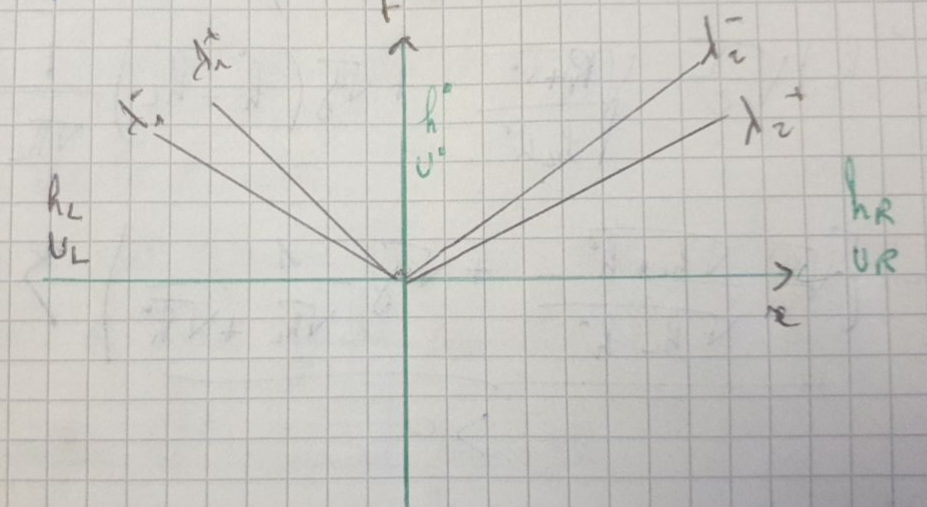
\includegraphics[scale=0.4]{Images_Fichiers/Y9.png}
%\legend{template}
%\label{1CCG}
\end{figure}

on distingue deux cas pour chaque i-onde:
\begin{itemize}
\item $\lambda^-_{i} < \lambda^+_{i}$:
Cas onde simple (i-d\'etente).
\item $\lambda^-_{i} = \lambda^+_{i}$:
Cas de i-choc.
\end{itemize}

et la vitesse du choc est:

$$\sigma = u + \frac{\lambda}{h}$$

La m\'ethode se r\'esume en 3 \'etapes:
\begin{itemize}
\item calcule de $hs = h^*$ (Newton)

On d\'eduit $u^*$ selon les \'equation en dessus pour les cas 1-choc et 2-choc.
\item $\lambda^{-,+}_{1,2}$ (1-choc et 2-choc)

Dans cette partie en utilise les invariants de Riemann. L'invariant de Riemann $R$ est rech\'erch\'e sous la forme:
$$u+fct(h)$$
avec la condition de $w -> R(w)$ i-invariant de Riemann ssi:
 $$\nabla R . r_i = 0$$

$r_i$ est le i\`eme vecteur propre qui d\'efinis par convention aussi la i\`eme choc.

\item On test $\frac{x}{t}$ avec les vitesses d'ondes.

\end{itemize}
Voici le code comment\'e de la r\'esolution du probl\`eme fourni ci-dessous:

\begin{lstlisting}
void riem_stvenant(double *wL, double *wR, double xi, double *w) {

  double g = 9.81;

  double hL = wL[0];
  double uL = wL[1]/wL[0];

  double hR = wR[0];
  double uR = wR[1]/wR[0];

  double hs = 1e-6;
  int itermax = 10;

  //on applique newton pour r\'esoudre f'(hs) = 0
  for (int i = 0; i < itermax; ++i){
    double f = uL - (hs - hL) * Z(hs, hL) - uR - (hs - hR) * Z(hs, hR);
    double df = -(hs - hL) * dZ(hs, hL) - Z(hs, hL) - (hs - hR) * dZ(hs,hR) - Z(hs,hR);
    double dhs = -f / df;
    hs += dhs;

    // printf("i=%d f=%e df=%e hs=%e dhs=%e \n", i, f, df, hs, dhs);
  }

  double us = uL - (hs - hL) * Z(hs, hL);

  double v1m, v1p, v2m, v2p;

  // 1 - onde
  if (hs < hL){ // détente

    v1m = uL - sqrt(g*hL);
    v1p = us - sqrt(g*hs);

  } else { // choc

    double a = sqrt(hs) / (sqrt(hs) + sqrt(hL));
    double u = a * us + (1 - a) * uL;
    double h = (hs + hL) / 2;

    v1m = u - sqrt(g*h); //relation 
    v1p = v1m;

  }

  // 2 - onde
  if (hs < hR){ // détente

    v2m = us + sqrt(g*hs);
    v2p = uR + sqrt(g*hR);

  } else { // choc

    double a = sqrt(hs) / (sqrt(hs) + sqrt(hR));
    double u = a * us + (1 - a) * uR;
    double h = (hs + hR) / 2;

    v2m = u + sqrt(g*h);
    v2p = v2m;

  }

  // printf("v = %f %f %f %f\nhs=%f us=%f\n", v1m, v1p, v2m, v2p, hs, us);

  if (xi < v1m){

    w[0] = wL[0];
    w[1] = wL[1];

  } else if (xi < v1p) {

    double u = (uL + 2*xi + 2*sqrt(g * hL)) / 3;
    double h = (u - xi) * (u - xi) / g;

    w[0] = h;
    w[1] = h * u;

  } else if (xi < v2m) {

    w[0] = hs;
    w[1] = hs * us;

  } else if (xi < v2p) {

    double u = (uR + 2*xi - 2*sqrt(g*hR)) / 3;
    double h = (u - xi) * (u - xi) / g;

    w[0] = h;
    w[1] = h * u;

  } else {

    w[0] = wR[0];
    w[1] = wR[1];

  }

}

\end{lstlisting}

\begin{figure}[h!]
	\centering 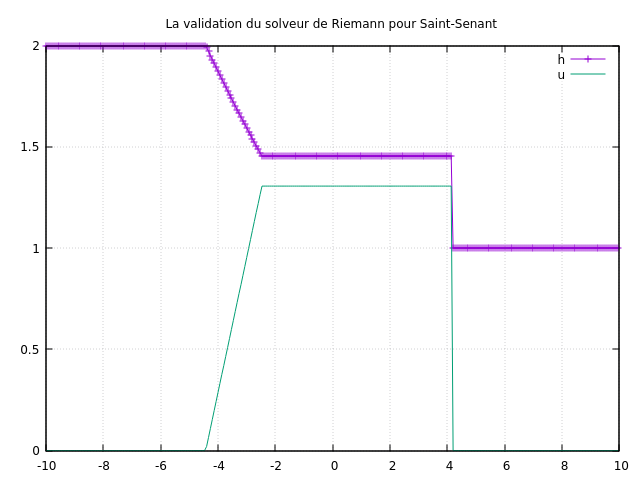
\includegraphics[scale=0.7]{Images_Fichiers/tp2q1.png}
%\legend{template}
%\label{1CCG}
\end{figure}
\newpage
\subsection[Programmer le sch\'ema de Godunov]{\uline{Programmer le sch\'ema de Godunov:}}

le sh\`ema de Godunov est bas\'e sur la discritisation suivante:

\begin{figure}[h!]
	\centering 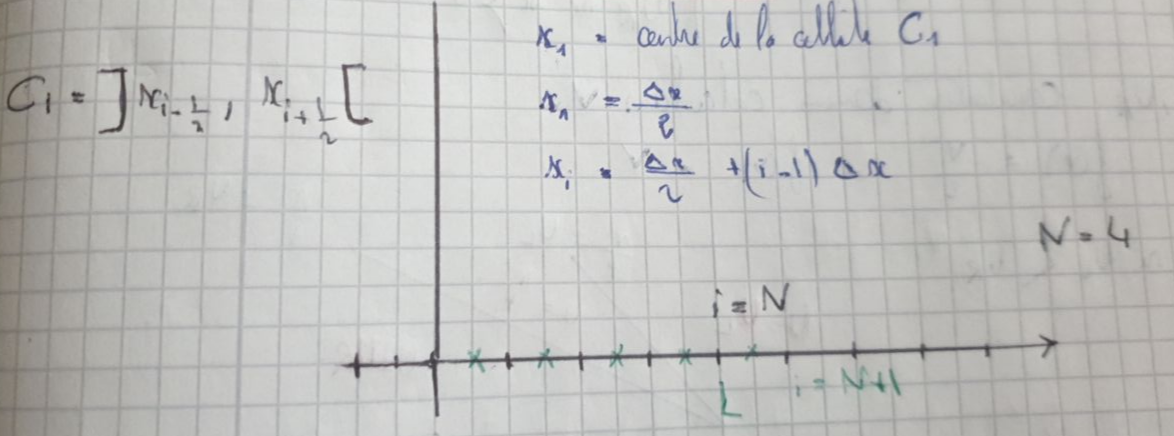
\includegraphics[scale=0.25]{Images_Fichiers/Y5.png}
%\legend{template}
%\label{1CCG}
\end{figure}
avec:

$$w_i = (h,hu)_i = u_i^n \sim u(x_i,t_n)$$

On rappel que le sch\'ema adopt\'e est:

$$ \frac {w_i^{n+1} -w_i^n}{\Delta t} + \frac {f(w_{i}^{n},w_{i+1}^{n}) - f(w_{i-1}^{n},w_{i}^{n})}{\Delta x} = 0$$ 
Avec:
$f(w_L, w_R)$ est le flux num\'erique qui repose sur la r\'esolution du probl\`eme de Riemann suivant:

\begin{equation}
\label{systeme}
\left \lbrace \begin{array}{rl}
\partial_t w +  \partial_x F(w)= 0, & w = (h, hu), \; et \; F(w) = (h u,h u^2 + g \frac{h^2}{2}) \quad avec \; g = 9.81 m/s^2,  \\
u(x,0) = 0,  \\
& h(x,0) =
\left \lbrace \begin{array}{rl}
h_L = 2 & ~\text{si }  x < 0\\
h_R = 1 & ~\text{si }  x > 0
\end{array}\right.
\end{array}\right.
\end{equation}


Alors la solution est bas\'ee sur le m\^eme raisonnement qu'en question 1:

\begin{equation}
\label{R}
v(x,t)=
\left \lbrace \begin{array}{rl}
u_R & ~\text{si }  x\geq ct\\
u_L & ~\text{si }  x<ct
\end{array}\right.
\end{equation}

On note $$v(x,t) = R(w_L,u_R,\frac {x}{t})$$

Et on peut en d\'eduire le flux num\'erique par la formule suivante:

$$f(a,b) = F(R(a,b,0))$$

Le pas $\Delta t$ est bas\'e sur la formule:
$$\Delta t = CFL \times \frac{\Delta x}{\lambda_{max}}$$

avec $\lambda_{max}$ est la plus grande des valeurs propres:

$$\lambda_{max} = |u| + \sqrt[2]{g h}$$

l'impl\'ementation est disponible sur le lien Github suivant:

\url{https://github.com/youness-elh/TP_EDP2_CSMI2/tree/main/TP2}



\subsection[La condition aux limites d'un bassin]{\uline{La condition aux limites d'un bassin:}}

On consid\`ere un bassin $[−10, 10]$ ferm\`e. Le bassin est s\'epar\'e en deux parties \'egales gr\^ace \`a une paroi situ\'e en x = 0. \`a
l’instant t = 0, la partie gauche (respt. droite) est remplie avec de l’eau immobile à une hauteur $h_L$ (respt. $h_R$). \`a l’instant
t = 0, on retire la paroi. 
La condition aux limites qu'on a impos\'e en x = −10 et x = 10:

\begin{lstlisting}

	    // valeurs aux bords
        int i;
        double wb[2];
        double *wm;

        i = 0; // bord gauche
        wm = svf->wn + (i+1)*m;
        // etat miroir
        wb[0] = wm[0];
        wb[1] = - wm[1];
        wm = svf->wn + i*m;
        for(int iv = 0; iv < m; ++iv) wm[iv] = wb[iv];

        i = n + 1; // bord droite
        wm = svf->wn + (i-1) * m;
        // etat miroir
        wb[0] = wm[0];
        wb[1] = - wm[1];
        wm = svf->wn + i * m;
        for(int iv=0; iv<m; ++iv) wm[iv] = wb[iv];
        
\end{lstlisting}

Comme c'est indiqu\'e sur la partie condition aux limites, on a un effet mirroir gardant la m\^eme hauteur mais inversant le sens du mouvement de l'eau et donc la vitesse u. Ceci est fait en multipliant par un signe $'-'$ la vitesse au bords gauche et droite. 

Dans le cas ou le bassin est infini, cette condition doit \^etre enlev\'ee.

\subsection[\'Evolution de la surface d’eau au cours du temps]{\uline{\'Evolution de la surface d’eau au cours du temps:}}

On lance le code pour une CFL = 0.5 et on \'evalue pour plusieurs valeurs de temps maximal (i.e 0,0.1,0.5,1,2,3) et pour plusieurs valeurs de discritisation (i.e 100, 1000).

\begin{itemize}
\item Pour N = 100

\newpage

\begin{itemize}
\item Pour T = 0:

\begin{figure}[h!]
	\centering 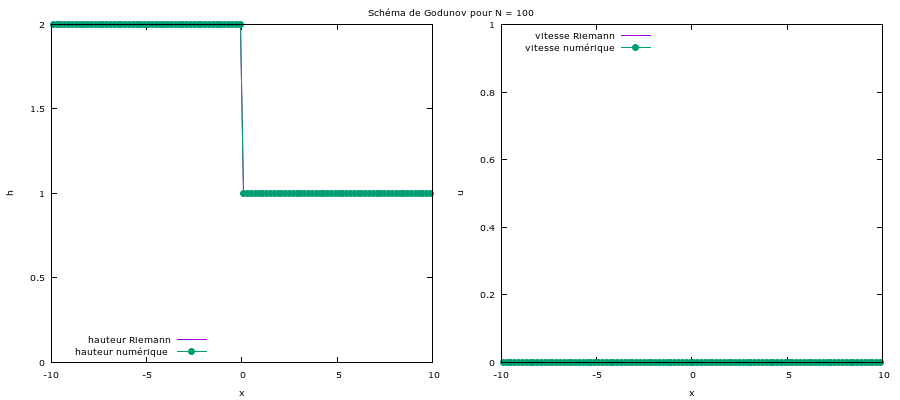
\includegraphics[scale=0.5]{Images_Fichiers/tp2godu100_0.png}
%\legend{template}
%\label{1CCG}
\end{figure}

\item Pour T = 0.1:

\begin{figure}[h!]
	\centering 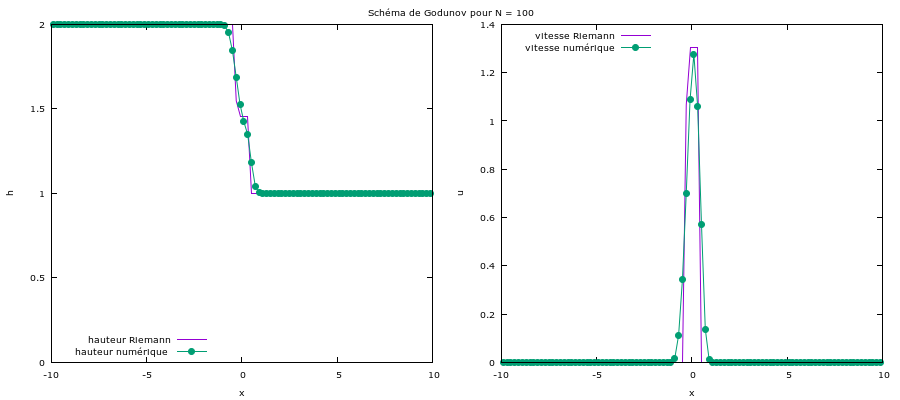
\includegraphics[scale=0.5]{Images_Fichiers/tp2godu100_01.png}
%\legend{template}
%\label{1CCG}
\end{figure}

\newpage
\item Pour T = 0.5:

\begin{figure}[h!]
	\centering 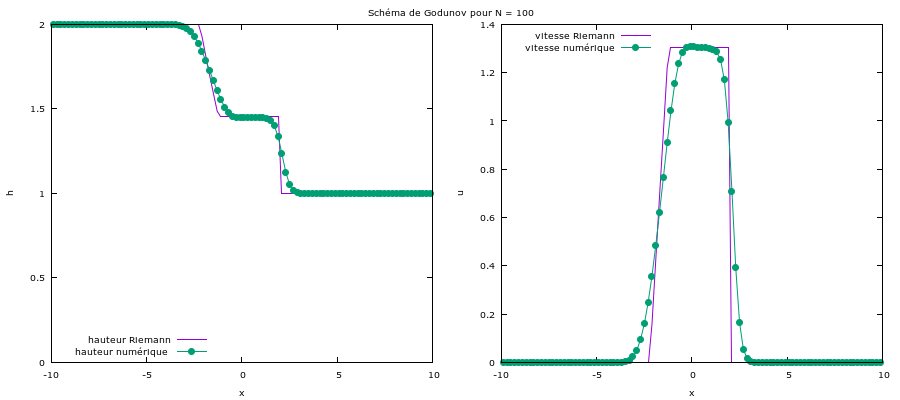
\includegraphics[scale=0.5]{Images_Fichiers/tp2godu100_05.png}
%\legend{template}
%\label{1CCG}
\end{figure}

\item Pour T = 1:

\begin{figure}[h!]
	\centering 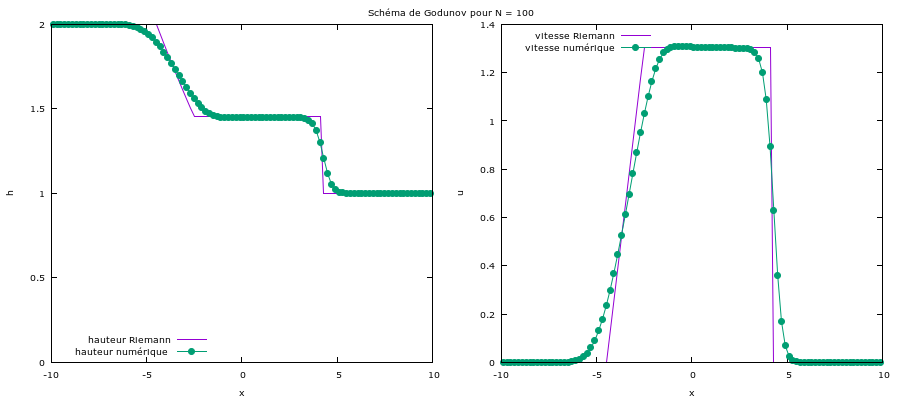
\includegraphics[scale=0.5]{Images_Fichiers/tp2godu100_1.png}
%\legend{template}
%\label{1CCG}
\end{figure}

\newpage
\item Pour T = 2:

\begin{figure}[h!]
	\centering 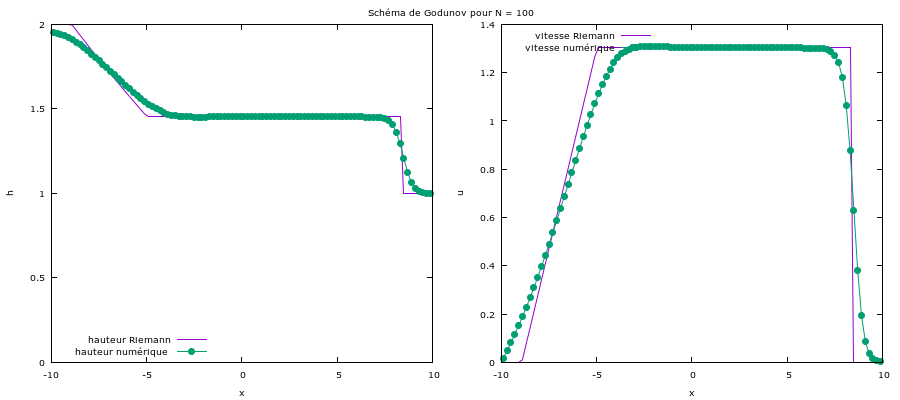
\includegraphics[scale=0.5]{Images_Fichiers/tp2godu100_2.png}
%\legend{template}
%\label{1CCG}
\end{figure}

\item Pour T = 3:

\begin{figure}[h!]
	\centering 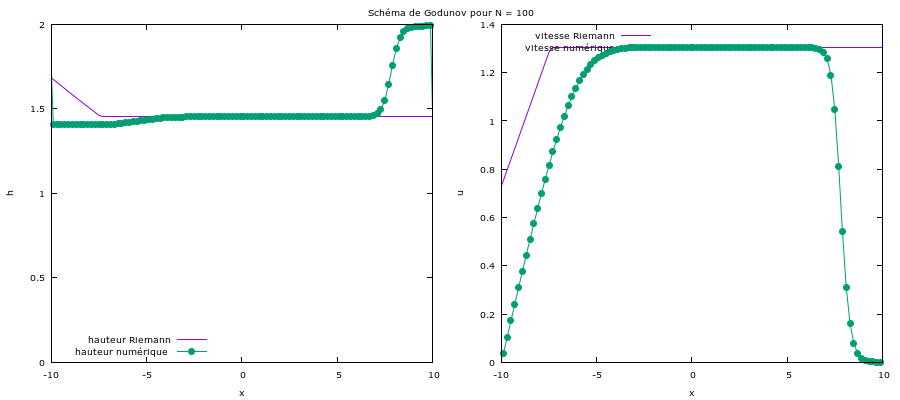
\includegraphics[scale=0.5]{Images_Fichiers/tp2godu100_3.png}
%\legend{template}
%\label{1CCG}
\end{figure}

\item Pour T = 4:

\begin{figure}[h!]
	\centering 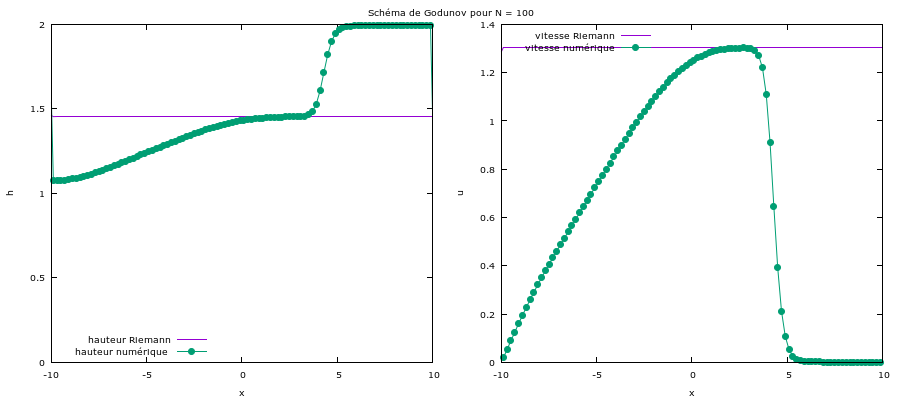
\includegraphics[scale=0.5]{Images_Fichiers/tp2godu100_4.png}
%\legend{template}
%\label{1CCG}
\end{figure}

\end{itemize}

\newpage

\item Pour N = 1000

\begin{itemize}
\item Pour T = 0:

\begin{figure}[h!]
	\centering 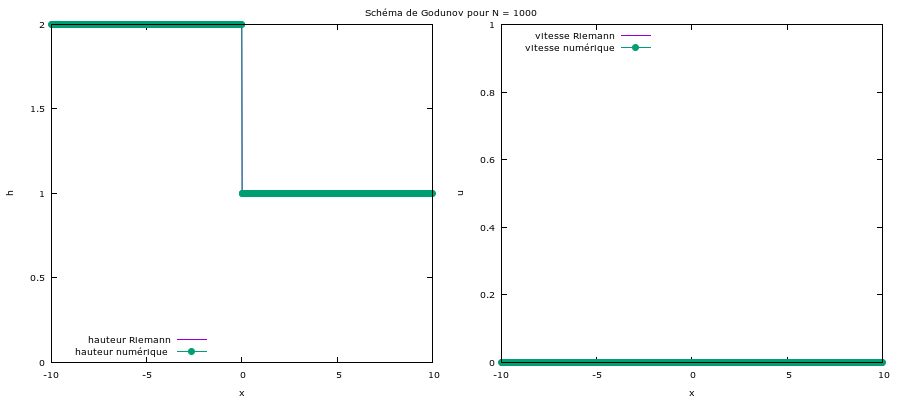
\includegraphics[scale=0.5]{Images_Fichiers/tp2godu1000_0.png}
%\legend{template}
%\label{1CCG}
\end{figure}

\item Pour T = 0.1:

\begin{figure}[h!]
	\centering 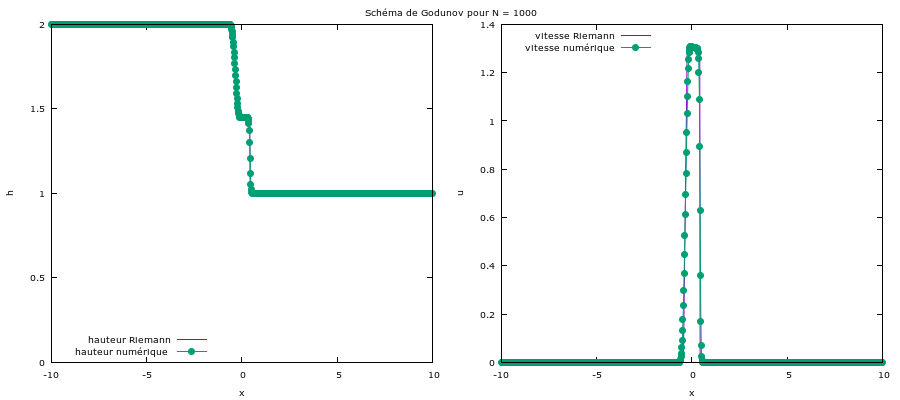
\includegraphics[scale=0.5]{Images_Fichiers/tp2godu1000_01.png}
%\legend{template}
%\label{1CCG}
\end{figure}

\newpage
\item Pour T = 0.5:

\begin{figure}[h!]
	\centering 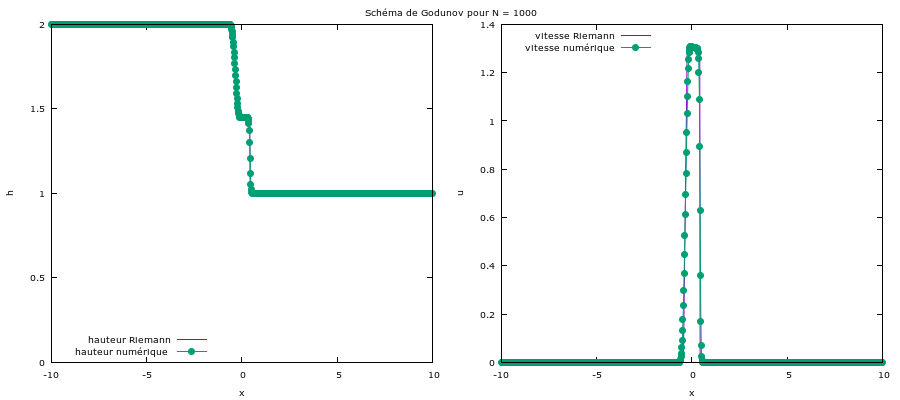
\includegraphics[scale=0.5]{Images_Fichiers/tp2godu1000_05.png}
%\legend{template}
%\label{1CCG}
\end{figure}

\item Pour T = 1:

\begin{figure}[h!]
	\centering 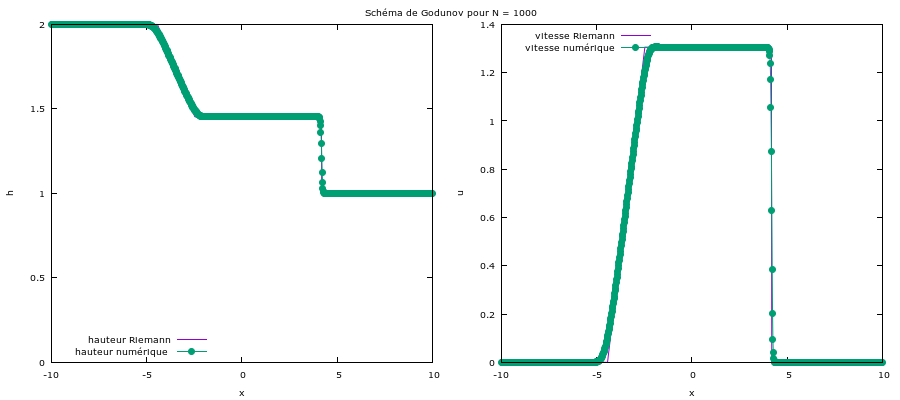
\includegraphics[scale=0.5]{Images_Fichiers/tp2godu1000_1.png}
%\legend{template}
%\label{1CCG}
\end{figure}

\newpage
\item Pour T = 2:

\begin{figure}[h!]
	\centering 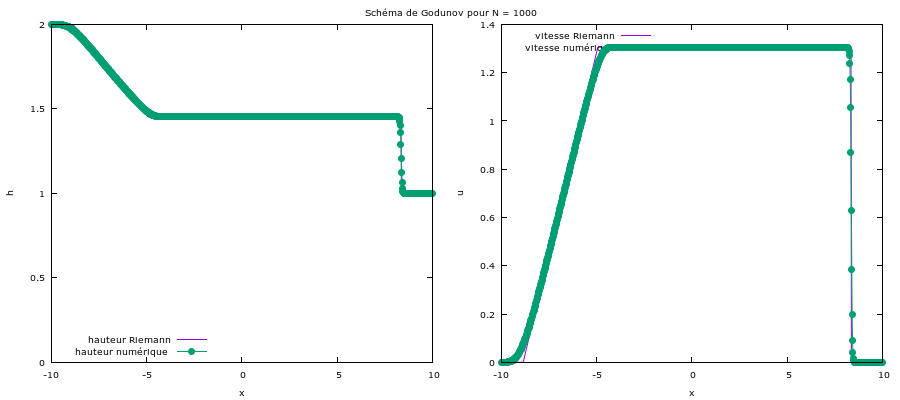
\includegraphics[scale=0.5]{Images_Fichiers/tp2godu1000_2.png}
%\legend{template}
%\label{1CCG}
\end{figure}

\item Pour T = 3:

\begin{figure}[h!]
	\centering 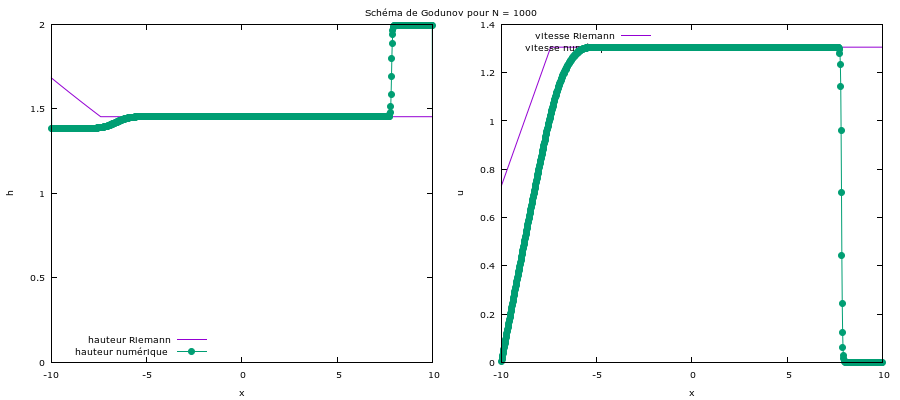
\includegraphics[scale=0.5]{Images_Fichiers/tp2godu1000_3.png}
%\legend{template}
%\label{1CCG}
\end{figure}

\newpage
\item Pour T = 4:

\begin{figure}[h!]
	\centering 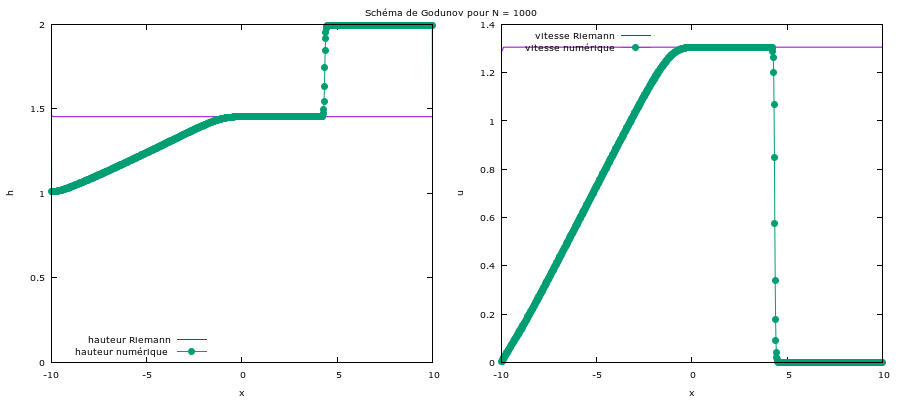
\includegraphics[scale=0.5]{Images_Fichiers/tp2godu1000_4.png}
%\legend{template}
%\label{1CCG}
\end{figure}

\end{itemize}


\end{itemize}

La solution num\'erique et proche de la solution exacte du probl\`eme de Riemann. Encore plus pour un grand nombre de discritisation N. Cependant, \`a partir d'un instant $T \sim 3$, il est plus claire que l'approximation Godunov n'est plus proche de la solution exacte Riemann. Ceci est d\^u au ratio $\frac{x}{t}$ qui devient plus petit quand tmax est grand et donc $< \lambda (w_L)$ engeandrant une solution constante $=w_L$.

\subsection[Le sch\'ema de Rusanov]{\uline{Le sch\'ema de Rusanov:}}

Le sch\'ema Rusanov n'est pas bas\'e sur le solveur Riemann quant \`a lui, contrairement \`a Godunov. La diff\'erence est donc dans le calcul du flux num\'erique qui est dans le cas Rusanov:

$$f(a,b) = \frac{F(a) + F(b)}{2} - \frac{\lambda(a,b)(b-a)}{2}$$

avec F est le flux physique et $\lambda(a,b)$ se calcule par la formule:

$$\lambda(a,b) = max(|F'(a)|,|F'(b)|)$$

On test pour une CFL = 0.5 et un nombre de descritisation N = 1000.

\begin{itemize}

\item Pour T = 0:

\begin{figure}[h!]
	\centering 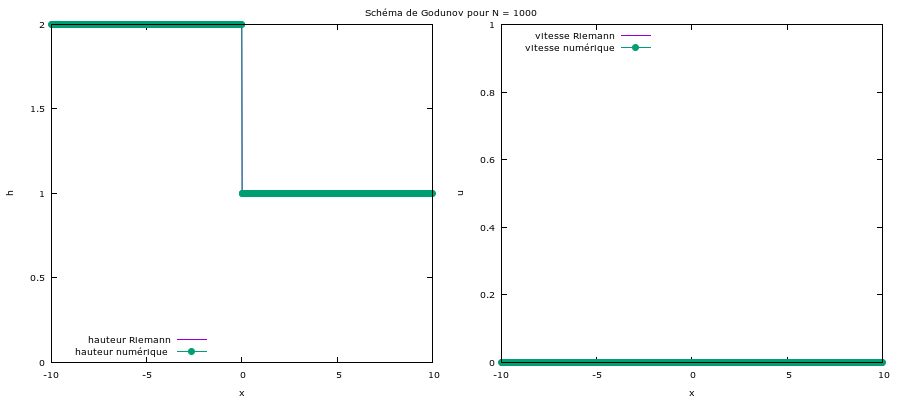
\includegraphics[scale=0.5]{Images_Fichiers/tp2rusa000_0.png}
%\legend{template}
%\label{1CCG}
\end{figure}

\item Pour T = 1:

\begin{figure}[h!]
	\centering 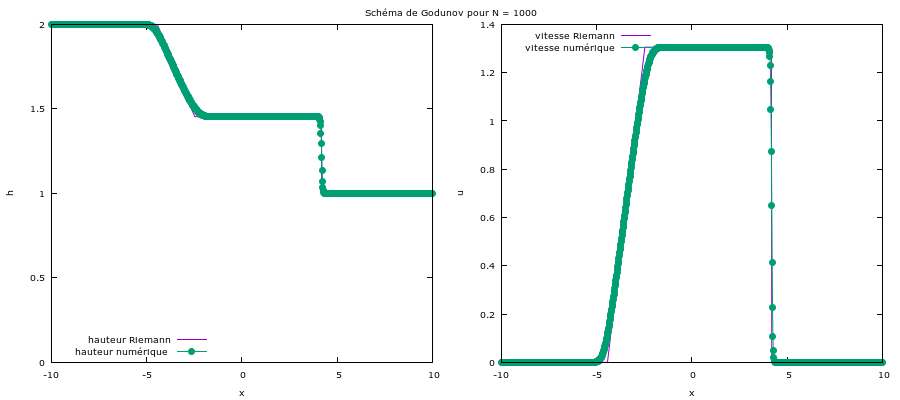
\includegraphics[scale=0.5]{Images_Fichiers/tp2rusa1000_1.png}
%\legend{template}
%\label{1CCG}
\end{figure}

\newpage
\item Pour T = 2:

\begin{figure}[h!]
	\centering 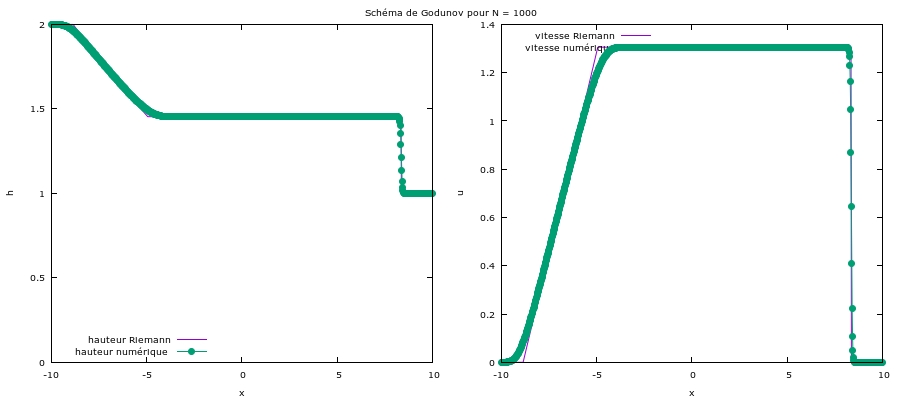
\includegraphics[scale=0.5]{Images_Fichiers/tp2rusa1000_2.png}
%\legend{template}
%\label{1CCG}
\end{figure}

\item Pour T = 3:

\begin{figure}[h!]
	\centering 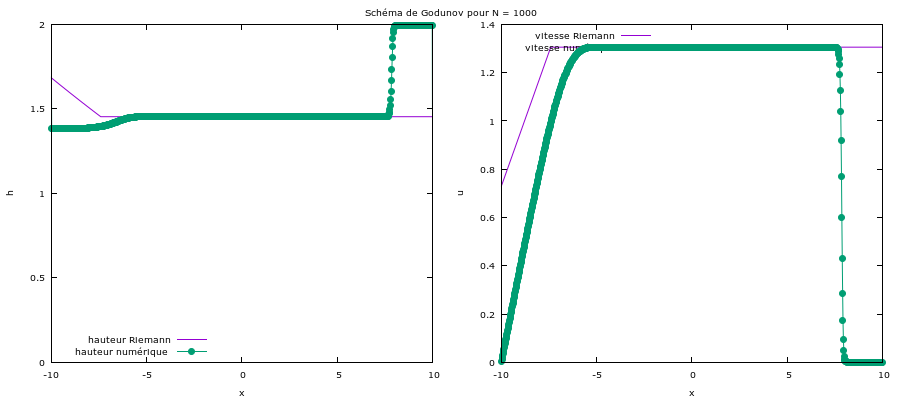
\includegraphics[scale=0.5]{Images_Fichiers/tp2rusa1000_3.png}
%\legend{template}
%\label{1CCG}
\end{figure}

\item Pour T = 4:

\begin{figure}[h!]
	\centering 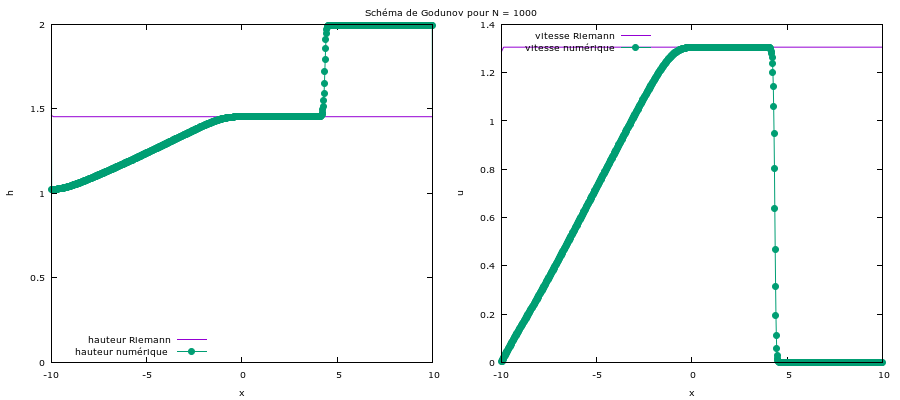
\includegraphics[scale=0.5]{Images_Fichiers/tp2rusa1000_4.png}
%\legend{template}
%\label{1CCG}
\end{figure}

\end{itemize}

\newpage

La m\'ethode Rusanov est bien plus rapide (un solveur de Riemann de moins), mais est elle pr\'ecise? les graphes suivant sont des graphes d'erreur $L^1$ de l'approximation Rusanov en premier temps puis Godunov de la hauteur en fonction du pas de descritisation $\Delta x$ pour un instant $T = 0.5$.

\begin{figure}[h!]
	\centering 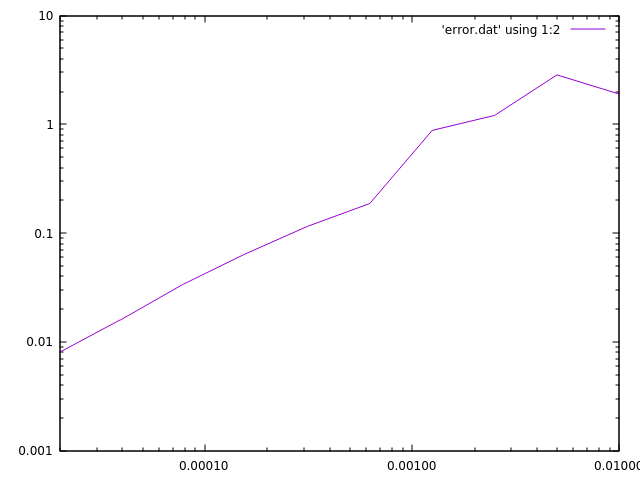
\includegraphics[scale=0.5]{Images_Fichiers/rusaerror_05.png}
	\centering 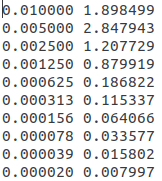
\includegraphics[scale=0.5]{Images_Fichiers/table_rusa.png}
%\legend{template}
%\label{1CCG}
\end{figure}

Et la figure suivante repr\'esente l'erreur L1 de la hauteur de Godunov, aussi pour un instant $T = 0.5$ et un $\Delta x$ variant entre $0.01$ et $1e-5$.
\newpage
\begin{figure}[h!]
	\centering 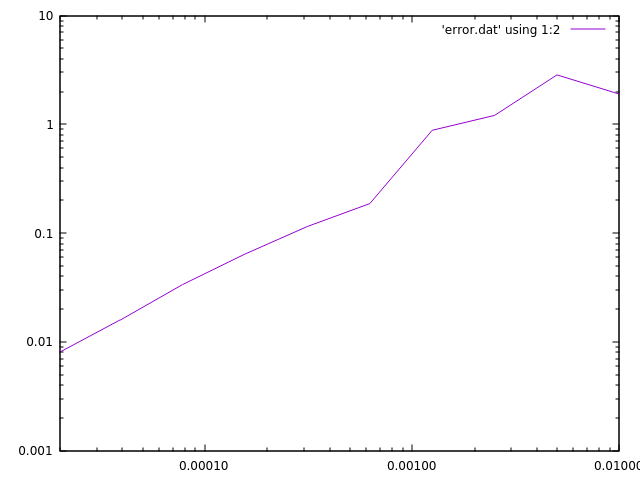
\includegraphics[scale=0.5]{Images_Fichiers/errorgodu100_05.png}
	\centering 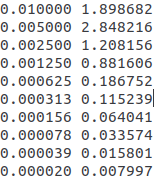
\includegraphics[scale=0.5]{Images_Fichiers/table_godu.png}
%\legend{template}
%\label{1CCG}
\end{figure}

On trace les deux erreur dans le m\^eme graphe.

\begin{figure}[h!]
	\centering 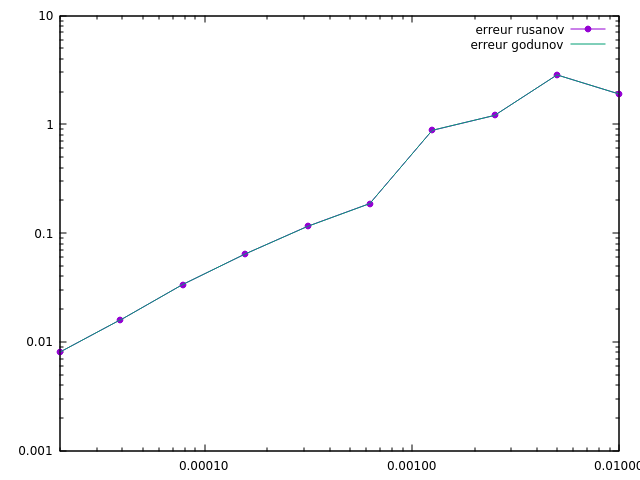
\includegraphics[scale=0.5]{Images_Fichiers/error_rusa_godu.png}

%\legend{template}
%\label{1CCG}
\end{figure}

L'erreur Rusanov est l\'egerement plus grande que celle produite par Godunov, aussi la valeur d'erreur atteinte en $\Delta x = 1e-5$ et plus petite pour Godunov donc on peut donc conclure que la m\'ethode Rusanov est moins pr\'ecise que Godunov.

\subsection[D\'ecrire le sch\'ema VFRoe et le flux num\'erique]{\uline{D\'ecrire le sch\'ema VFRoe et le flux num\'erique:}}

L'id\'ee du sch\'ema de VFRoe est de remplacer le solveur de Riemann exact par un solveur de Riemann approch\'e, plus rapide et plus simple.

On rappel que le sch\'ema adopt\'e est:

$$ \frac {w_i^{n+1} -w_i^n}{\Delta t} + \frac {f(w_{i}^{n},w_{i+1}^{n}) - f(w_{i-1}^{n},w_{i}^{n})}{\Delta x} = 0$$ 
Avec:
$f(w_L, w_R)$ est le flux num\'erique qui repose sur la r\'esolution du probl\`eme de VFRoe $\tilde{R}$.

$$f(w_L, w_R) = F(\tilde{R}(w_L,w_R,0))$$

On a:

$$w_t + F(w)_x = 0 \quad (*)$$

avec w = (h,hu)

En posant $y = \begin{pmatrix}
h\\
u
\end{pmatrix} \; (*) \iff$

$$y_t + B(y)y_x = 0 \quad avec \; B(y) = \begin{pmatrix}
u & h \\
g & u 
\end{pmatrix}$$ 

avec $
y
\begin{pmatrix}
h \\
u 
\end{pmatrix}
$ variables primitives.

On va lin\'eariser les \'equations autour d'un \'etat moyen.

$$\tilde{y} = \frac{y_L+y_R}{2}$$

On remplace la r\'esolution du probl\`eme Riemann par:

\begin{equation}
\label{systeme}
\left \lbrace \begin{array}{rl}
y_t +  B(\tilde{y})y_x= 0, \\
& y(x,0) =
\left \lbrace \begin{array}{rl}
y_L  & ~\text{si }  x < 0\\
y_R  & ~\text{si }  x > 0
\end{array}\right.
\end{array}\right.
\end{equation}

et on utilise la formule:

$$ y(0,t) = \tilde{y} - sign(B(\tilde{y})) \times \tilde{y}$$

On d\'etermine le signe de $B(\tilde{y})$ en utilisant le polyn\^ome d'interpolation Q de la fonction g sur les valeurs propres de B.

On pose:

$\lambda_1 = \tilde{u}-\sqrt{g \tilde h}$ et $\lambda_2 = \tilde{u} + \sqrt{g \tilde h}$ les valeurs propres de $B(\tilde{y})$.
$$B = PDP^{-1}$$
$$g(B):= P\begin{pmatrix}
g(\lambda_1) & 0 \\
0 & g(\lambda_2) 
\end{pmatrix}P^{-1}$$
$$Q(\lambda_1) = g(\lambda_1), \quad
Q(\lambda_2) = g(\lambda_2), \quad et \; d°Q = 1$$
$$Q(B) = g(B)$$

Soit $$B(\tilde y) = \begin{pmatrix}
\tilde u & \tilde h \\
g & \tilde u 
\end{pmatrix}$$

soit : $\tilde{c} = \sqrt{g \tilde h}$ 
Et on distingue 3 cas pour calculer le signe de $B(\tilde y)$:

\begin{itemize}
\item cas $\lambda_1$ et $\lambda_2$ sont $>0$:

$$sign(B(\tilde y) ) = I$$

alors: $$y(0,t) = y_L$$

Et donc:
$$\tilde{R}(w_L,w_R,0) = w_L$$

\item cas $\lambda_1$ et $\lambda_2$ sont $<0$:

$$sign(B(\tilde y) ) = -I$$

alors: $$y(0,t) = y_R$$

Et donc:
$$\tilde{R}(w_L,w_R,0) = w_R$$

\item cas $\lambda_1 < 0$ et $\lambda_2 > 0$:
On d\'efinie Q:
si $\lambda = \lambda_1$  alors $Q(\lambda) = -1$

si $\lambda = \lambda_2$  alors $Q(\lambda) = 1$

et donc: $$Q(\lambda) = -1\frac{\lambda-\lambda_2}{\lambda_1-\lambda_2} + 1\frac{\lambda-\lambda_1}{\lambda_1-\lambda_2} = \frac{\lambda - \tilde{u}}{\tilde{c}}$$

alors:

$$sign(B(\tilde y) ) = Q(B(\tilde y) ) =  \frac{B - \tilde{u}I}{\tilde{c}} $$
$$ = \frac{1}{\tilde c} \begin{pmatrix}
0 & \tilde h \\
g & 0 
\end{pmatrix}$$

donc:
$$ y(0,t) = \tilde{y} - \frac{1}{\tilde c} \begin{pmatrix}
0 & \tilde h \\
g & 0 
\end{pmatrix} \times \tilde{y}$$

On a donc les varibles primitives:

$$ h^* = \frac{h_L + h_R}{2} - \frac{1}{2\sqrt{g \tilde{h}}} \tilde{h}(u_R -u_L)$$
$$ u^* = \frac{u_L + u_R}{2} - \frac{1}{2\sqrt{g \tilde{h}}} g (h_R -h_L)$$

Et donc:
$$\tilde{R}(w_L,w_R,0) = w(y(0,t))$$

\end{itemize}

Et on d\'eduit le flux num\'erque pour chacun des cas expliqu\'e en dessus.

$$f(w_L,w_R) = F(\tilde{R}(w_L,w_R,0)) $$

 

\subsection[Programmer le sch\'ema VFRoe]{\uline{Programmer le sch\'ema VFRoe:}}

Le code qui mis en oeuvre le flux num\'erique calcul\'e en dessus est le suivant:

\begin{lstlisting}
void vfroe_stvenant(double *wL, double *wR, double xi, double *w) {

  double g = 9.81;

  double hL = wL[0];
  double uL = wL[1]/wL[0];

  double hR = wR[0];
  double uR = wR[1]/wR[0];


  double uc = (uR + uL)/2;
  double hc = (hL + hR)/2;

  double cc = sqrt(g*hc);

  double lbd1 = uc - cc;
  double lbd2 = uc + cc;

  double h, u;
  if (lbd1 < 0 && lbd2 < 0){
      h = hR;
      u = uR;
  }
  else if (lbd1 > 0 && lbd2 > 0) {
      h = hL;
      u = uL;
  } else {
      h = hc*(1 - (uR - uL)/cc);
      u = uc - g*(hR - hL)/2/cc;
  }
  w[0] = h;
  w[1] = h*u;

}
        
\end{lstlisting}

Pour v\'erifier que ce sch\'ema ne donne pas toujours la bonne solution on choisit un probl\'eme de Riemann associ\'e \`a une onde de d\'etente qui traverse une valeur propre nulle. Dans cette d\'etente, $u+ 2\sqrt {gh}$ est constant et l’onde contient un point $u-2\sqrt {gh} = 0$.

En effet on prend les conditions aux limites suivants:

\begin{lstlisting}

    double hL = 1.;
    double uL = -1.;

    double hR = 1./4;
    double uR = uL + 2*sqrt(9.81) * (sqrt(hL)-sqrt(hR));
    
\end{lstlisting}

Et on a donc une fausse approximation de la partie de discontinuit\'e:

\begin{figure}[h!]
	\centering 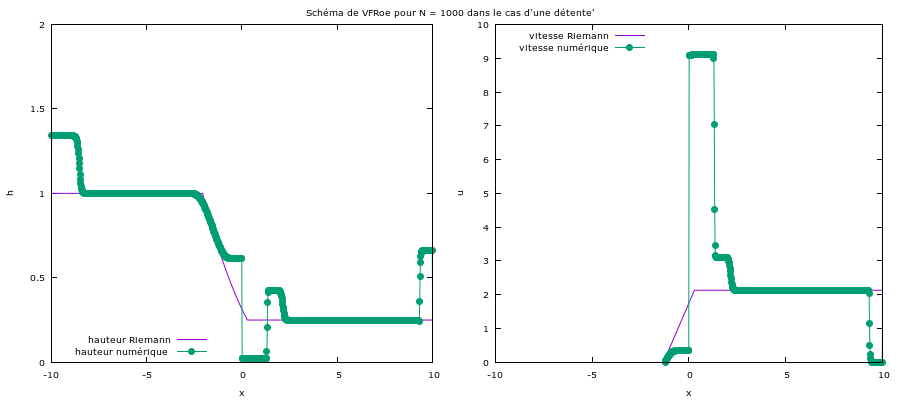
\includegraphics[scale=0.5]{Images_Fichiers/vfroe1.png}

%\legend{template}
%\label{1CCG}
\end{figure}

alors que pour un cas de deux ondes ca fonctionne correctement.

\begin{figure}[h!]
	\centering 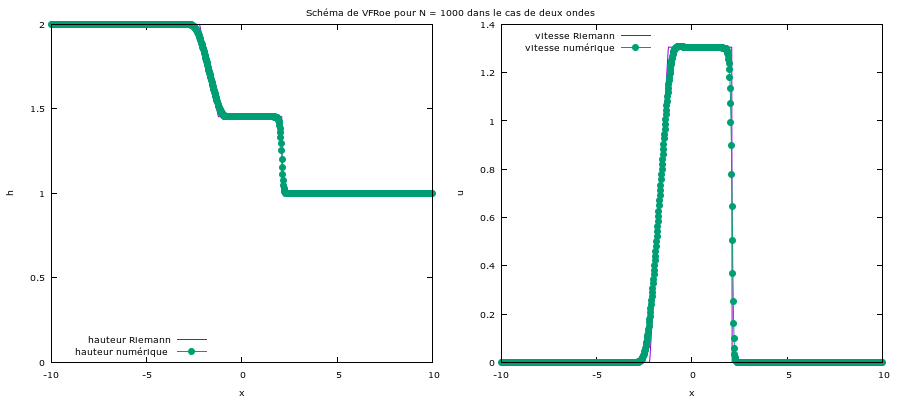
\includegraphics[scale=0.5]{Images_Fichiers/vfroe2.png}

%\legend{template}
%\label{1CCG}
\end{figure}

\subsection[Programmer la correction entropique qui utilise le flux de Rusanov aux points “soniques”]{\uline{Programmer la correction entropique qui utilise le flux de Rusanov aux points “soniques”:}}

\subsection[Comparer avec le sch\'ema Godunov]{\uline{Comparer avec le sch\'ema Godunov:}}

\subsection[Le sch\'ema de Roe]{\uline{Le sch\'ema de Roe:}}

\subsection[La correction MUSCL de van Leer]{\uline{la correction MUSCL de van Leer:}}



